\documentclass{article}
\usepackage{setspace}
\usepackage[margin=.8 in]{geometry}
\usepackage{amsmath,graphicx}
\usepackage[font=small,skip=1pt]{caption}
\usepackage{float}
\captionsetup[figure]{font=small,skip=1pt}
\author{\#Authors}
\title{Stereo odometry based on  Local Intensity Order Pattern}
\onehalfspacing
\begin{document}
\maketitle
\begin{abstract}
New generation autonomous vehicles use different data fusion techniques to solve the Simultaneous Localization And Mapping (SLAM) problems in urban terrains.  However, the majority of the implementations uses high-cost sensors like LIDAR to obtain a high accuracy map. In this paper, we  present a novel method  to solve this problem using sequences of stereo images. Our approach uses Local Intensity Order Pattern (LIOP) based  feature descriptors to  overcome the problem of monotonic intensity changes and affine transformations of detected features. Egomotion of the vehicle is estimated using correspondence of features on the consecutive frames. Estimated motion parameters are then corrected using an extended Kalman filter. Depth of the detected features is calculated using stereo triangulation. Mahalanobis distance  is used to avoid outliers in the detected features.
The accuracy of  the proposed method is  evaluated using the measurements from a  high accurate inertial navigation system. Method is tested using the odometry data set of the KITTI Vision Benchmark Suite.
			
\end{abstract}
\section{Introduction}

 Precise  pose estimation is  the key prerequisite for  achieving autonomous driving of any mobile robotics systems. However, commonly dead-reckoning methods are prone to accumulation of error over time. In this work, we concentrate on a method called visual odometry, which uses a  camera to estimate the position of the vehicle. In order to calculate 6DOF camera motion, the system has to detect and match the features between the image frames. Depth of the features is obtained using triangular geometry between  image views and the camera baseline. Main contribution of this paper  as follows.

\begin{itemize}
\item Use of a feature descriptor which is invariant to photometric transformations.
\item Outlier rejection scheme based on Mahalanobis distance.
\end{itemize}
\par
Our experimental results shows, rotational error at high speed will be reduced significantly by the use of  proposed feature descriptor, which is invariant to  photometric transformations such as image blur. 

\section{Related Literature}

Visual odometry has been gaining attention of the research community over the last few years. Several methods have been proposed to compute the ego-motion using stereo \cite{mandelbaum1999correlation}, \cite{mallet2000position}, \cite{Kitt2010IV}, \cite{badino2013visual} and the monocular \cite{bruss1983passive}, \cite{heeger1992subspace}, \cite{kanatani19933} \cite{wagner1999robust} sequence of images. Hernan Badino and et al. \cite{badino2013visual} propose a Method to reduce the projection error by computing the optical flow  over all past frames. Ji Zhang et al. \cite{zhang2014real} explores use of bundle adjustment to increase the accuracy. Efficient use of GPU-based pipelines to optimize a  binocular bundle adjustment algorithm is suggested by Wei Lu et al. \cite{hpvo}.

\par
Error model in stereo navigation system is proposed by Matthies et al. \cite{matthies1987error}. Their experiments showed that  3D Gaussian reduces the variance in robot position. However, in order to have a high accurate position estimation, system have to incorporate an invariant feature detection and representation method.  Scaramuzza et al. \cite{Scaramuzza2008} uses SIFT based feature description methods to achieve a better accuracy. Bernd Kitt et al. \cite{Kitt2010IV} recommends the use of RANSAC based outlier  rejection  scheme with a feature bucketing technique to select better feature points.


\section{System Overview}

The proposed system is similar to the method suggested by Bernd Kitt et al.\cite{Kitt2010IV}. However, to make the system more robust to illumination changes, specular reflection and blur   LIOP \cite{wang2011local} based  feature descriptors are introduced. To Mahalanobis distance-based outlier rejection \cite{Blanco2012} method is are used to calculate optimal correspondence between the feature points. Shortlisted feature points are projected to 3D with the help of triangulation from the camera baseline to obtain the depth. Estimated camera motion parameters are corrected using   the extended Kalman filter. An overview of the system is given in fig \ref{sv}.
\begin{figure}[ht]
 \centering
 \includegraphics[width=10cm]{images/so.eps}
\caption{System Overview}
\label{sv}
\end{figure}

\subsection{Feature extraction, description and matching }
The performance of a visual odometry system  depends on extraction and representation of features. To achieve a consistent odometry in adverse weather and lighting conditions, the descriptor must be invariant to photometric transforms such as  specular reflections, complex illumination changes and monotonic intensity changes.
However, the widely used descriptors such as Scale Invariant Feature Transform(SIFT) and Gradient Location-Orientation Histogram (GLOH) are robust to geometric transformations but sensitive to  photometric transformations.
\par
The proposed system uses  Local Intensity Order Pattern(LIOP)\cite{wang2011local} based descriptors to encode  the regions detected by the Hessian-affine covariant region detector. In the preprocessing stage, image is smoothed by a Gaussian filter and feature position and shape are identified by the Hessian-affine detector\cite{mikolajczyk2002affine}. Detected regions are normalized to circular areas of fixed diameter. These local patches are sorted based on the intensity level of the pixels and construct a histogram based on the order. 

\par
Rotation invariant is achieved by taking neighbourhood pixels of pixel $x$ in the anticlockwise direction on a circle. In order to develop  the histogram, the identified order of intensities in the neighbourhood  of pixels will map to a linear index. Bins are constructed based on the weighted pooling of mapped linear indices  in the region. Extracted features are matched using the fast nearest neighbour matching algorithm. Figure \ref{match} shows randomly selected feature matches .

\begin{figure}[ht]
 \centering
 \includegraphics[width=15cm , height=4cm]{images/matchc.eps}
\caption{LIOP descriptor matches between  left and right images.}
\label{match}
\end{figure}
\subsection{Outlier rejection and State Estimation}
Mahalanobis distance is used to identify the optimal set of the detected feature matches. It is used to calculate the distance between a feature and the overall distribution of the feature correspondence. The Mahalanobis distance \cite{de2000mahalanobis} of an observation $x = ( x_1, x_2, x_3, \dots, x_N )^T$ from a group of observations with mean $\mu = ( \mu_1, \mu_2, \mu_3, \dots , \mu_N )^T$ and covariance matrix $S$ is defined as:

\begin{equation}D_M(x) = \sqrt{(x - \mu)^T S^{-1} (x-\mu)}.\end{equation}

These features are projected to 3D using the triangular geometry between the image views and camera baseline with help of camera intrinsic parameters. This process is repeated over image frames to measure the motion of the camera. Estimated motion parameter are corrected using an extended Kalman filter.

\section{Results and Observations}
Proposed method is tested using KITTI vision benchmark suite\cite{Geiger2012CVPR}  and estimated position  and errors for the sequence-01 are given in figure [3-7]. Algorithms are implemented using C++ with help of VLFEAT library in an  i5-3210M, 2.5Ghz CPU.Following are the observations from this empirical method.

\begin{itemize}
\item Use of LIOP based feature descriptors will improve the accuracy of the estimation, but the computational cost is high. 
\item  LIOP features are invariant to the photometric transformation such as illumination changes. However, It can be further improved in the context of visual odometry.
\end{itemize}
\begin{figure}[ht]
 \centering
 \includegraphics[width=10cm ]{images/01.eps}
\caption{Estimated path.}
\label{match}
\end{figure}
\begin{figure}[H]
    \centering
    \begin{minipage}{.5\textwidth}
    
        \centering
        \includegraphics[width=8cm]{images/01_rl.eps}
        \vspace{-1.5em}
        \caption{Rotation Error  vs Path Length}
        \label{a}
    \end{minipage}%
    \begin{minipage}{0.5\textwidth}
        \centering
        \includegraphics[width=8cm]{images/01_rs.eps}
         \vspace{-1.5em}
        \caption{Rotation Error  vs Speed}
        \label{b}
    \end{minipage}
    \centering
    \begin{minipage}{.5\textwidth}
        \centering
        \includegraphics[width=8cm]{images/01_tl.eps}
         \vspace{-1.5em}
        \caption{Translation Error  vs Path Length}
        \label{c}
    \end{minipage}%
    \begin{minipage}{0.5\textwidth}
        \centering
        \includegraphics[width=8cm]{images/01_ts.eps}
         \vspace{-1.5em}
        \caption{Translation Error  vs Speed}
        \label{fd}
    \end{minipage}
\end{figure}
\section{conclusion}
 In this paper, we presented a method to estimate ego-motion using visual odometry. This technique relies on  LIOP based feature detector.
Majority of the data set available to evaluate the system does not include the images in a bad weather condition or night driving. So this method needs to explore further with the help of more challenging image datasets with specular reflections and complex illumination changes. 

\bibliographystyle{IEEEbib}
\bibliography{ref}
\end{document}

